{$\vx = \bmx{c}1\\1\emx$, $\vy = \bmx{c} -2\\3\emx$}
{$\vx+\vy = \bmx{c}-1\\4\emx$, $\vx-\vy = \bmx{c} 3\\-2\emx$

Sketches will vary depending on choice of origin of each vector.

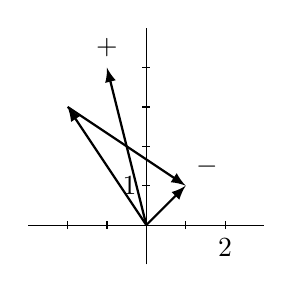
\begin{tikzpicture}[>=latex,scale=.5]
% Draw grid
\draw (-3,0)--(3,0);
\draw (0,-1)--(0,5);
\foreach \x in {-2,...,2}
 {\draw (\x,-.1)--(\x,.1);
 }
\foreach \x in {1,...,4}
 {\draw (-.1,\x)--(.1,\x);
 };
\node[below] at (2,-0.1) {2};
\node[left] at (0,1) {1};
%Draw arrows
\draw [->,thick] (0,0)--(1,1) node [below] {\vx};
\draw [->,thick] (0,0) -- (-2,3) node [below left] {\vy};
\draw [->,thick] (0,0) -- (-1,4) node [above] {$\vx+\vy$};
\draw [->,thick] (-2,3) -- (1,1) node [above right] {$\vx-\vy$};
\end{tikzpicture}
}